\chapter{Podstawy teoretyczne}

\section{Uczenie maszynowe i reinforcement learning}

Uczenie maszynowe (ang. Machine Learning, ML) to dziedzina sztucznej inteligencji, która pozwala wybranemu algorytmowi na automatyczne uczenie się wzorców z danych bez potrzeby jawnego określania parametrów wewnętrznych. Przykładem uczenia maszynowego jest dostosowanie parametrów funkcji liniowej do zbioru danych:

\[
f(x) = ax + b,
\]

gdzie \(a\) (nachylenie) i \(b\) (przecięcie z osią Y) są parametrami, które należy dostosować tak, aby funkcja najlepiej przybliżała dane wejściowe. Proces ten polega na minimalizacji różnicy między wartościami przewidywanymi przez model a rzeczywistymi wartościami w zbiorze danych. Problemy poruszane przez uczenie maszynowe zwykle są związane z bardzo dużą liczbą parametrów.

\subsection{Podstawowe pojęcia}

Uczenie ze wzmocnieniem opiera się na kluczowych pojęciach: 
\begin{itemize}
    \item \textbf{Agent} – model; podmiot podejmujący decyzje na podstawie obserwowanego stanu środowiska.
    \item \textbf{Środowisko (ang. Environment)} – otoczenie, w którym agent działa i z którym wchodzi w interakcje.
    \item \textbf{Stan (ang. State)} – opis bieżącej sytuacji środowiska, obserwowany przez agenta.
    \item \textbf{Akcja (ang. Action)} – decyzja podejmowana przez agenta, wpływająca na środowisko.
    \item \textbf{Nagroda (ang. Reward)} – liczba, która ocenia efektywność podjętej akcji w danym stanie.
\end{itemize}

Uczenie maszynowe można podzielić na trzy główne kategorie:

\begin{itemize}
    \item \textbf{Uczenie nadzorowane (ang. Supervised Learning)} – model jest trenowany na zestawie danych, które zawierają zarówno wejścia (ang. inputs), jak i odpowiadające im wyjścia (ang. outputs). Celem jest nauczenie modelu przewidywania wyjścia dla nowych, nieznanych danych na podstawie znanych znanych par wejścia-wyjścia (np. opis obrazka).

    \item \textbf{Uczenie nienadzorowane (ang. Unsupervised Learning)} – dane treningowe zawierają jedynie wejścia, bez przypisanych wyjść. Algorytm stara się odkrywać ukryte wzorce lub grupy w danych.

    \item \textbf{Uczenie ze wzmocnieniem (ang. Reinforcement Learning)} – agent uczy się przez interakcję ze środowiskiem, podejmując akcje, które maksymalizują otrzymywaną nagrodę. W odróżnieniu od uczenia nadzorowanego, nie ma bezpośrednio dostępnych par wejście-wyjście – agent musi odkryć najlepszą strategię działania na podstawie prób i błędów.
\end{itemize}

\subsection{Algorytm Double Q-Learning}

Double Q-Learning jest ulepszeniem klasycznego algorytmu Q-Learning, który pozwala agentowi uczyć się optymalnej strategii (ang. policy) w środowiskach opartych na nagrodach. Kluczowym problemem tradycyjnego Q-Learningu jest ryzyko przeszacowywania wartości \( Q(s, a) \), co może prowadzić do błędnych decyzji w złożonych środowiskach. Double Q-Learning minimalizuje to ryzyko, wykorzystując dwie oddzielne tablice wartości \( Q_1 \) i \( Q_2 \), które są aktualizowane naprzemiennie.

\paragraph{Podstawy algorytmu Q-Learning:}
W tradycyjnym Q-Learningu agent aktualizuje wartość \( Q(s, a) \) według równania Bellmana:

\[
Q(s, a) \leftarrow Q(s, a) + \alpha \left( r + \gamma \max_{a'} Q(s', a') - Q(s, a) \right),
\]

gdzie:
\begin{itemize}
    \item \( Q(s, a) \) – aktualna wartość dla stanu \( s \) i akcji \( a \),
    \item \( \alpha \) – współczynnik uczenia, który kontroluje szybkość aktualizacji,
    \item \( r \) – nagroda za podjęcie akcji \( a \),
    \item \( \gamma \) – współczynnik dyskontowy, określający znaczenie przyszłych nagród,
    \item \( \max_{a'} Q(s', a') \) – maksymalna wartość Q dla następnego stanu \( s' \) przy dowolnej akcji \( a' \).
\end{itemize}

\paragraph{Ulepszenie w Double Q-Learning:}
Double Q-Learning dzieli wartości \( Q \) na dwie tablice: \( Q_1 \) i \( Q_2 \). Przy każdej aktualizacji wybierana jest losowo jedna z tych tablic do aktualizacji, podczas gdy druga tablica jest wykorzystywana do wyboru optymalnej akcji. Aktualizacja wartości \( Q \) przebiega według następującego schematu:

1. Jeśli wybrano tablicę \( Q_1 \):
\[
Q_1(s, a) \leftarrow Q_1(s, a) + \alpha \left( r + \gamma Q_2(s', \arg\max_{a'} Q_1(s', a')) - Q_1(s, a) \right),
\]

2. Jeśli wybrano tablicę \( Q_2 \):
\[
Q_2(s, a) \leftarrow Q_2(s, a) + \alpha \left( r + \gamma Q_1(s', \arg\max_{a'} Q_2(s', a')) - Q_2(s, a) \right).
\]

Wykorzystanie dwóch tablic pozwala na bardziej wiarygodne szacowanie wartości akcji, ponieważ wybór optymalnej akcji jest niezależny od tablicy, która aktualizuje wartości.

\paragraph{Zalety Double Q-Learning:}
\begin{itemize}
    \item Redukcja przeszacowań wartości \( Q(s, a) \), co poprawia stabilność uczenia.
    \item Lepsze działanie w środowiskach o dużej zmienności, takich jak gry wideo.
    \item Zachowanie prostoty implementacji, ponieważ wymaga jedynie rozdzielenia tablic \( Q \).
\end{itemize}

\paragraph{Zastosowanie w grze Super Mario Bros:}
W projekcie Double Q-Learning jest używany do nauki optymalnej strategii dla postaci Mario, bazując na danych odczytywanych z pamięci emulatora. Tablice \( Q_1 \) i \( Q_2 \) przechowują wartości akcji takich jak ruch w lewo, w prawo, skok czy bieg, w zależności od aktualnego stanu gry, reprezentowanego m.in. przez pozycję Mario i stany przeszkód.

\section{Architektura gry Super Mario Bros (NES)}

Super Mario Bros to gra platformowa, w której każdy poziom można traktować jako sekwencję stanów i akcji, co czyni ją idealnym środowiskiem do zastosowania uczenia ze wzmocnieniem.

\subsection{Struktura gry}

Gra składa się z następujących elementów:
\begin{itemize}
    \item \textbf{Poziomy (ang. Levels)} – każdy poziom zawiera przeszkody, przeciwników i cele do osiągnięcia.
    \item \textbf{Stan gry (ang. Game State)} – opisuje bieżącą pozycję Mario, czas, liczbę żyć, punkty oraz inne parametry.
    \item \textbf{Akcje (ang. Actions)} – gracz (lub model) może sterować postacią Mario za pomocą ruchów (w lewo, w prawo, skoków) oraz akcji specjalnych (np. ataku).
\end{itemize}

\subsection{Struktura pamięci emulatora}

Dane o stanie gry są przechowywane w pamięci emulatora NES. Kluczowe informacje, które można odczytać, to:
\begin{itemize}
    \item Pozycja Mario (\texttt{mario\_x}, \texttt{mario\_y}),
    \item Stan życia (\texttt{lives}),
    \item Liczba punktów (\texttt{score}),
\end{itemize}


\begin{figure}[h!]
    \centering
    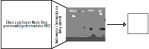
\includegraphics[width=0.5\textwidth]{img/schemat_nes.svg}
    \caption{miau}
    \label{fig:nes_controller}
\end{figure}

